% Options for packages loaded elsewhere
\PassOptionsToPackage{unicode}{hyperref}
\PassOptionsToPackage{hyphens}{url}
%
\documentclass[
]{article}
\usepackage{amsmath,amssymb}
\usepackage{lmodern}
\usepackage{iftex}
\ifPDFTeX
  \usepackage[T1]{fontenc}
  \usepackage[utf8]{inputenc}
  \usepackage{textcomp} % provide euro and other symbols
\else % if luatex or xetex
  \usepackage{unicode-math}
  \defaultfontfeatures{Scale=MatchLowercase}
  \defaultfontfeatures[\rmfamily]{Ligatures=TeX,Scale=1}
\fi
% Use upquote if available, for straight quotes in verbatim environments
\IfFileExists{upquote.sty}{\usepackage{upquote}}{}
\IfFileExists{microtype.sty}{% use microtype if available
  \usepackage[]{microtype}
  \UseMicrotypeSet[protrusion]{basicmath} % disable protrusion for tt fonts
}{}
\makeatletter
\@ifundefined{KOMAClassName}{% if non-KOMA class
  \IfFileExists{parskip.sty}{%
    \usepackage{parskip}
  }{% else
    \setlength{\parindent}{0pt}
    \setlength{\parskip}{6pt plus 2pt minus 1pt}}
}{% if KOMA class
  \KOMAoptions{parskip=half}}
\makeatother
\usepackage{xcolor}
\usepackage{graphicx}
\makeatletter
\def\maxwidth{\ifdim\Gin@nat@width>\linewidth\linewidth\else\Gin@nat@width\fi}
\def\maxheight{\ifdim\Gin@nat@height>\textheight\textheight\else\Gin@nat@height\fi}
\makeatother
% Scale images if necessary, so that they will not overflow the page
% margins by default, and it is still possible to overwrite the defaults
% using explicit options in \includegraphics[width, height, ...]{}
\setkeys{Gin}{width=\maxwidth,height=\maxheight,keepaspectratio}
% Set default figure placement to htbp
\makeatletter
\def\fps@figure{htbp}
\makeatother
\setlength{\emergencystretch}{3em} % prevent overfull lines
\providecommand{\tightlist}{%
  \setlength{\itemsep}{0pt}\setlength{\parskip}{0pt}}
\setcounter{secnumdepth}{-\maxdimen} % remove section numbering

%%%% pandoc-fignos: required package
\usepackage{caption}

%% pandoc-fignos: environment to disable figure caption prefixes
\makeatletter
\newcounter{figno}
\newenvironment{fignos:no-prefix-figure-caption}{
  \caption@ifcompatibility{}{
    \let\oldthefigure\thefigure
    \let\oldtheHfigure\theHfigure
    \renewcommand{\thefigure}{figno:\thefigno}
    \renewcommand{\theHfigure}{figno:\thefigno}
    \stepcounter{figno}
    \captionsetup{labelformat=empty}
  }
}{
  \caption@ifcompatibility{}{
    \captionsetup{labelformat=default}
    \let\thefigure\oldthefigure
    \let\theHfigure\oldtheHfigure
    \addtocounter{figure}{-1}
  }
}
\makeatother
\ifLuaTeX
  \usepackage{selnolig}  % disable illegal ligatures
\fi
\IfFileExists{bookmark.sty}{\usepackage{bookmark}}{\usepackage{hyperref}}
\IfFileExists{xurl.sty}{\usepackage{xurl}}{} % add URL line breaks if available
\urlstyle{same} % disable monospaced font for URLs
\hypersetup{
  pdftitle={Lab 1},
  hidelinks,
  pdfcreator={LaTeX via pandoc}}

\title{Lab 1}
\author{}
\date{}

\begin{document}
\maketitle

\hypertarget{goals}{%
\section{Goals}\label{goals}}

In this lab, you will use basic test and measurement equipment that are
useful for building and testing electronic circuits. In particular, you
will make measurements of voltage using an oscilloscope and digital
multimeter. You will also determine an accurate measurement technique
for measuring small resistances.

Proficiency with new equipment

\begin{itemize}
\item
  DC Power Supply:

  \begin{itemize}
  \item
    Set up the connections to supply both (+) and (-) voltage
  \item
    Operate in voltage controlled and current controlled modes
  \end{itemize}
\item
  Oscilloscope:

  \begin{itemize}
  \item
    Measure DC voltage levels
  \item
    Determine the effects of DC and AC input coupling
  \item
    Determine the effects of changing the input impedance
  \item
    Trigger the scope on different waveforms
  \end{itemize}
\item
  Function generator:

  \begin{itemize}
  \item
    Create various shaped waveforms, and modify amplitude and frequency
  \item
    Change the output impedance to match the rest of your system
  \end{itemize}
\item
  Digital Multimeter (DMM):

  \begin{itemize}
  \item
    Measure DC voltages and DC currents
  \item
    Determine the frequency and impedance limitations of the DMM
  \end{itemize}
\end{itemize}

Experimental design

\begin{itemize}
\item
  Develop familiarity with the model-based approach to experiment
\item
  Measuring small resistances using a 4-terminal approach
\end{itemize}

\hypertarget{lab-notebook-guidelines}{%
\section{Lab Notebook Guidelines}\label{lab-notebook-guidelines}}

The lab notebook will play an essential role in this course. You will
use your notebook for keeping records of many things including:

\begin{itemize}
\item
  Answering lab-prep questions from the lab guide
\item
  Answering in-lab questions
\item
  Recording data
\item
  Including plots of data
\item
  Analysis and results
\item
  Diagrams and pictures
\item
  Procedures of experiments that you design
\end{itemize}

The lab notebook will be an important part of your grade because
learning to keep a good lab notebook is an important part of your
professional development. You may find it helpful to write up many of
your notes on the computer, for example, within Mathematica or another
program. This is fine. However, before your notebook is turned in, the
notes, plots, and analysis should be transferred to the lab notebook by
printing and taping the pages or keeping them in a three-ring binder.
This is standard practice in research labs. Your lab notebook is the
main mechanism for communicating your process and results of the lab
experiments. Each week, you will be responsible for turning in both your
pre-laboratory work and your lab notebook / analysis via Canvas in
scanned format. See the syllabus for more information.

\hypertarget{definitions}{%
\section{Definitions}\label{definitions}}

\textbf{Power rail (or rail)} - this refers to the ± V power supply
outputs that powers the circuit.

\textbf{Electrical Load} \textbf{(or load)} - this refers to the circuit
or impedance connected to the output of a circuit.

\textbf{RMS (Root Mean Square)} - is the square root of the average of a
periodic function squared over one period. Example: For the function
\(Y = A\ sin(\omega t)\), the RMS value is
\(\sqrt{\overline{Y^{2}}} =\ A/\sqrt{2}\).

\hypertarget{useful-readings}{%
\section{Useful Readings}\label{useful-readings}}

\begin{enumerate}
\def\labelenumi{\arabic{enumi}.}
\item
  \href{https://atomoptics-nas.uoregon.edu/~dsteck/teaching/electronics/electronics-notes.pdf}{Steck}
  - This text is freely available as a PDF, so you may want to download
  it and keep it handy. Sections 1.1 - 1.3.2 are appropriate for Lab 1.
\item
  Fischer-Cripps (FC) Chapters 1 (Electricity), 2 (DC Circuits), and 3
  (AC Circuits) introduce important topics relevant to the first two
  weeks of lecture. Note: we will revisit various sections in these
  chapters in more detail later - for example filters and oscillators.
  Also look at p.~274 for the resistor color code (or search for it on
  the internet).
\item
  Horowitz and Hill 2\textsuperscript{nd} Edition (H\&H) - Chapter 1,
  Sections 1.01-1.12
\item
  The following documents, which can be found on Canvas, will be useful:

  \begin{itemize}
  \item
    Keysight EDU33210 Series Waveform Generator User Guide and Data
    Sheet
  \item
    Keysight EDU36311A Power Supply User Guide (p.~43-45) and Data Sheet
  \item
    Tektronix TBS2000 Series Oscilloscope User Manual
  \item
    Math review on complex numbers
  \end{itemize}
\end{enumerate}

\hypertarget{setting-up-the-dc-power-supply}{%
\section{Setting up the DC Power
Supply}\label{setting-up-the-dc-power-supply}}

Your DC power supply will provide all of your circuits with the required
power. Setting up the power supply will always be the first thing you do
when you begin working with a circuit. The Keysight EDU36311A DC Power
Supply has three outputs that can be independently controlled. Pages
43-45 of the User Guide (which can be found on Canvas) discuss this in
detail.

\hypertarget{set-up-the-dc-voltage-bias}{%
\subsection{Set up the DC voltage
bias}\label{set-up-the-dc-voltage-bias}}

\begin{enumerate}
\def\labelenumi{\arabic{enumi}.}
\item
  We want two of the power supply channels to be set up such that the
  potential difference set on one of the channels is positive with
  respect to ground and the other is negative with respect to ground.
  Each channel has outputs labeled (+) and (-) and you will find that
  the single output connector to the left of Channel 1 is connected to
  chassis ground. The voltage indicated on the power supply display
  shows only the potential difference between the (+) and (-) output.
  You must connect the (-) to ground to get a positive voltage with
  respect to ground, and the (+) to ground to get a negative voltage
  with respect to ground. Since Channels 2 and 3 on the Keysight
  EDU36311A Power Supply have the equivalent output voltage and current
  specifications, it makes the most sense to use these two channels (see
  Figure \ref{fig:ps}).
\item
  Confirm the sign and magnitude of the voltages displayed on the power
  supply using the DMM. In your lab notebook, document the setup, the
  output voltage from the power supply, and the measured output on your
  DMM. \emph{\textbf{Note:} Hooking up the power supply to your circuit
  with reversed polarity or to too high a voltage can cause your
  components to be destroyed.}
\end{enumerate}

\hypertarget{investigate-operating-modes}{%
\subsection{Investigate operating
modes}\label{investigate-operating-modes}}

A voltage source maintains a constant potential difference while the
current output varies dependent on the load resistance (this is the
Constant Voltage (CV) mode). A current source maintains a constant
current while the voltage output varies dependent on the load resistance
(this is the Constant Current (CC) mode). The power supply will indicate
the operational mode of each channel in the upper right corner of the
respective channel window (in addition to CV and CC modes, the other
mode is OFF).

\begin{enumerate}
\def\labelenumi{\arabic{enumi}.}
\item
  With no load attached, record the output voltage and current for both
  power rails (see definitions).
\item
  Try adjusting the value of the voltage and current. Why is the current
  output always zero?
\item
  Now short the (+) rail to ground. You can use a banana cable from the
  rack to do this.
\item
  Vary the value of the voltage and current. Describe the behavior of
  the voltage and current readings and the mode (CV/CC) of the power
  supply. What happens when you short the output to ground (have too
  small a load)? What is the maximum output of current and voltage your
  supply can produce?
\end{enumerate}

\begin{figure}
\hypertarget{fig:ps}{%
\centering
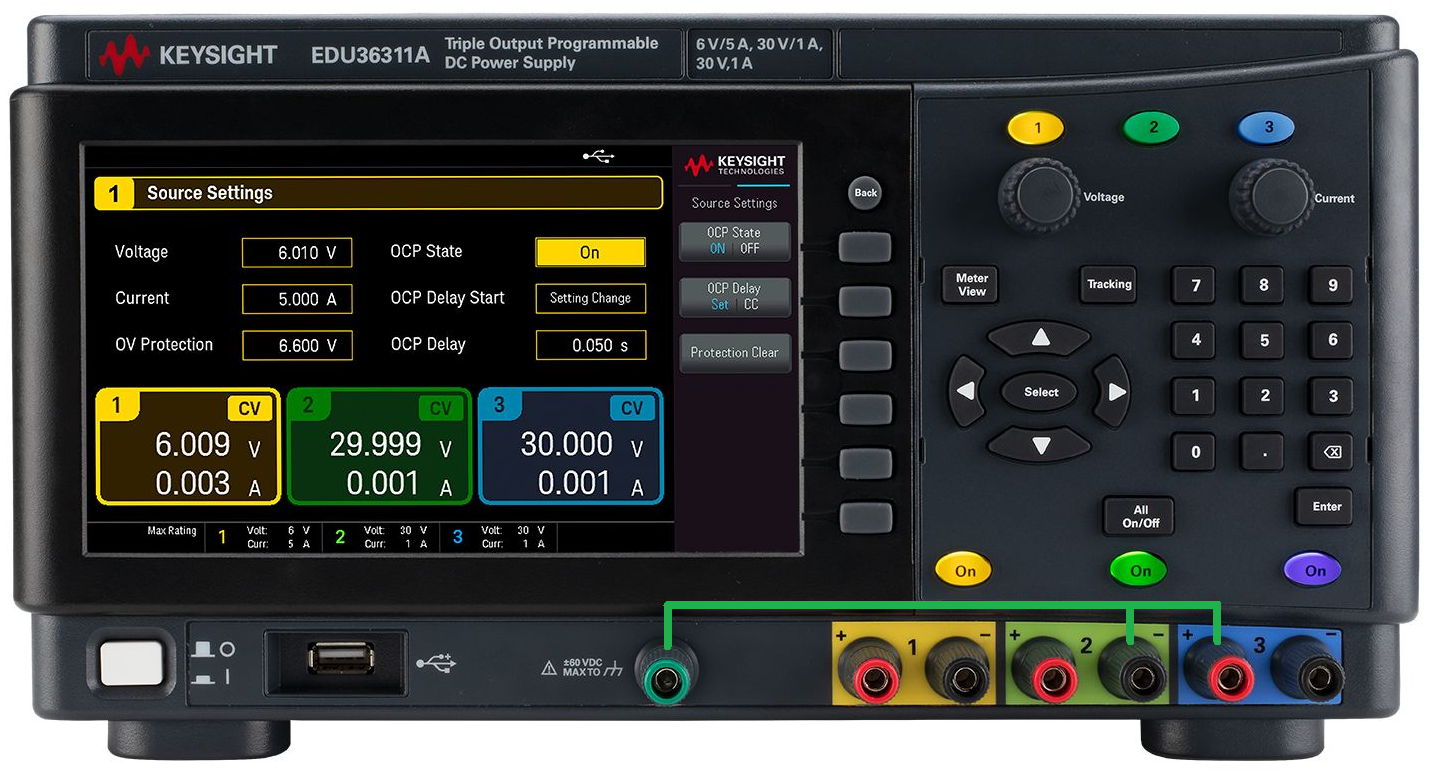
\includegraphics[width=20cm,height=\textheight]{https://raw.githubusercontent.com/kwbunker/PHYS-3330-Scratch/main/lab1fig/EDU36311A.png}
\caption{Keysight EDU36311A DC power supply connections}\label{fig:ps}
}
\end{figure}

\hypertarget{measuring-voltage-with-the-oscilloscope}{%
\section{Measuring Voltage with the
Oscilloscope}\label{measuring-voltage-with-the-oscilloscope}}

The goal of this part of the lab is to be able to use an oscilloscope
(frequently referred to as scope or o-scope) to make measurements of DC
voltages and AC waveforms. You will also learn how to produce various
waveforms using a function generator.

There are a few precautions to observe when operating the oscilloscope:

\begin{itemize}
\item
  Avoid overheating the instrument. Do not block ventilation of the
  interior.
\item
  Do not apply more than 300 V to any input terminal.
\item
  Avoid serious or fatal injury from electrical shock. Do not remove the
  cover to expose the 120 V mains.
\end{itemize}

Otherwise, the instruments are robust and cannot be damaged by wrong
settings. So, try whatever youre curious about and measure and document
what happens.

\hypertarget{measuring-a-dc-voltage-on-a-scope}{%
\subsection{Measuring a DC voltage on a
scope}\label{measuring-a-dc-voltage-on-a-scope}}

The Tektronix TBS 2000 Series has four independent channels so that four
separate signals can be displayed at once. Each trace is color coded
with the buttons on the panel.

\begin{enumerate}
\def\labelenumi{\arabic{enumi}.}
\item
  Connect a +5V signal from your power supply to the scope using the
  supplied connectors. Measure the voltage on scope using the cursors.
  Try exploring the different knobs and menus on the scope to make the
  measurement. Refer to the appendix listed at the end of this document
  if you get stuck.
\item
  In your lab notebook, describe the setup of the electric circuits
  (diagrams are useful) and the outcomes measured.
\end{enumerate}

\emph{NOTE: Oscilloscopes can only distinguish about 100 different
values on the vertical axes of the screen. So before you use the
oscilloscope to measure anything make sure that the trace covers at
least 50\% of the vertical screen without clipping at the top or bottom.
This way you get a resolution/accuracy of approximately ±2\%.}

\begin{figure}
\hypertarget{fig:bnc}{%
\centering
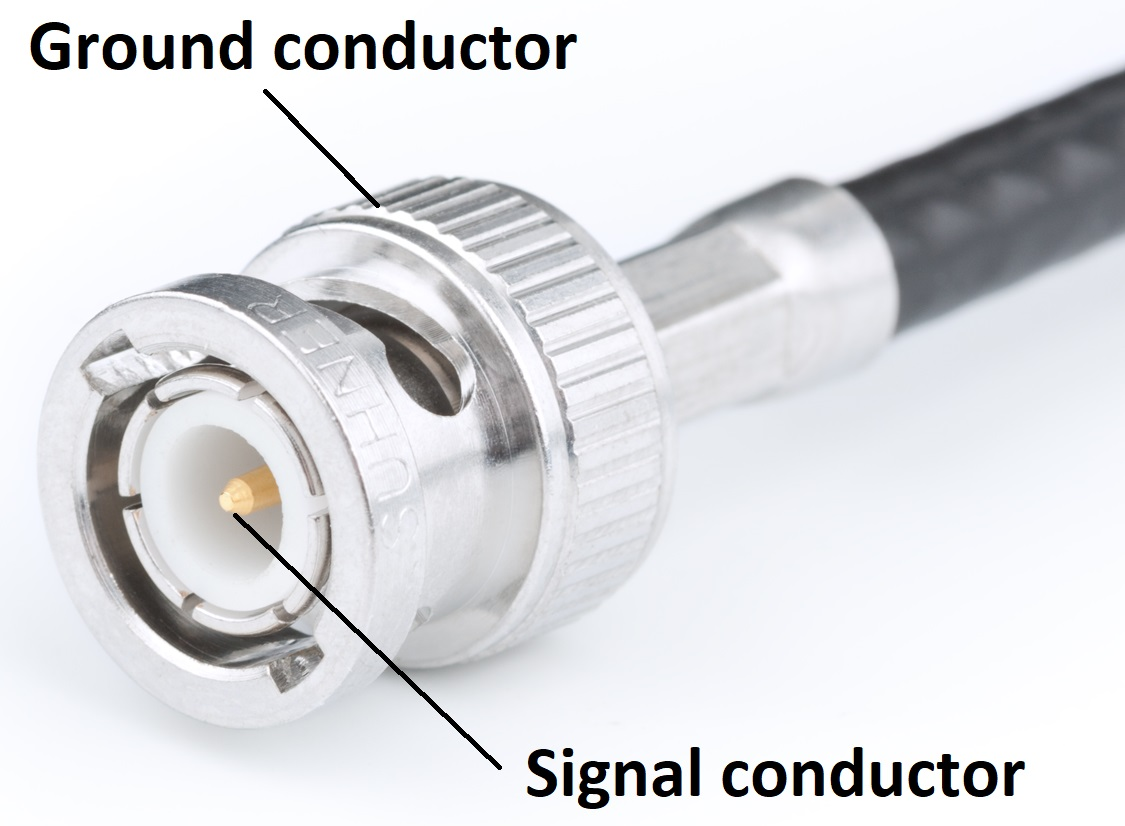
\includegraphics[width=10cm,height=\textheight]{https://raw.githubusercontent.com/kwbunker/PHYS-3330-Scratch/main/lab1fig/bnc-plug.jpg}
\caption{BNC Plug Connector}\label{fig:bnc}
}
\end{figure}

\begin{figure}
\hypertarget{fig:grabber}{%
\centering
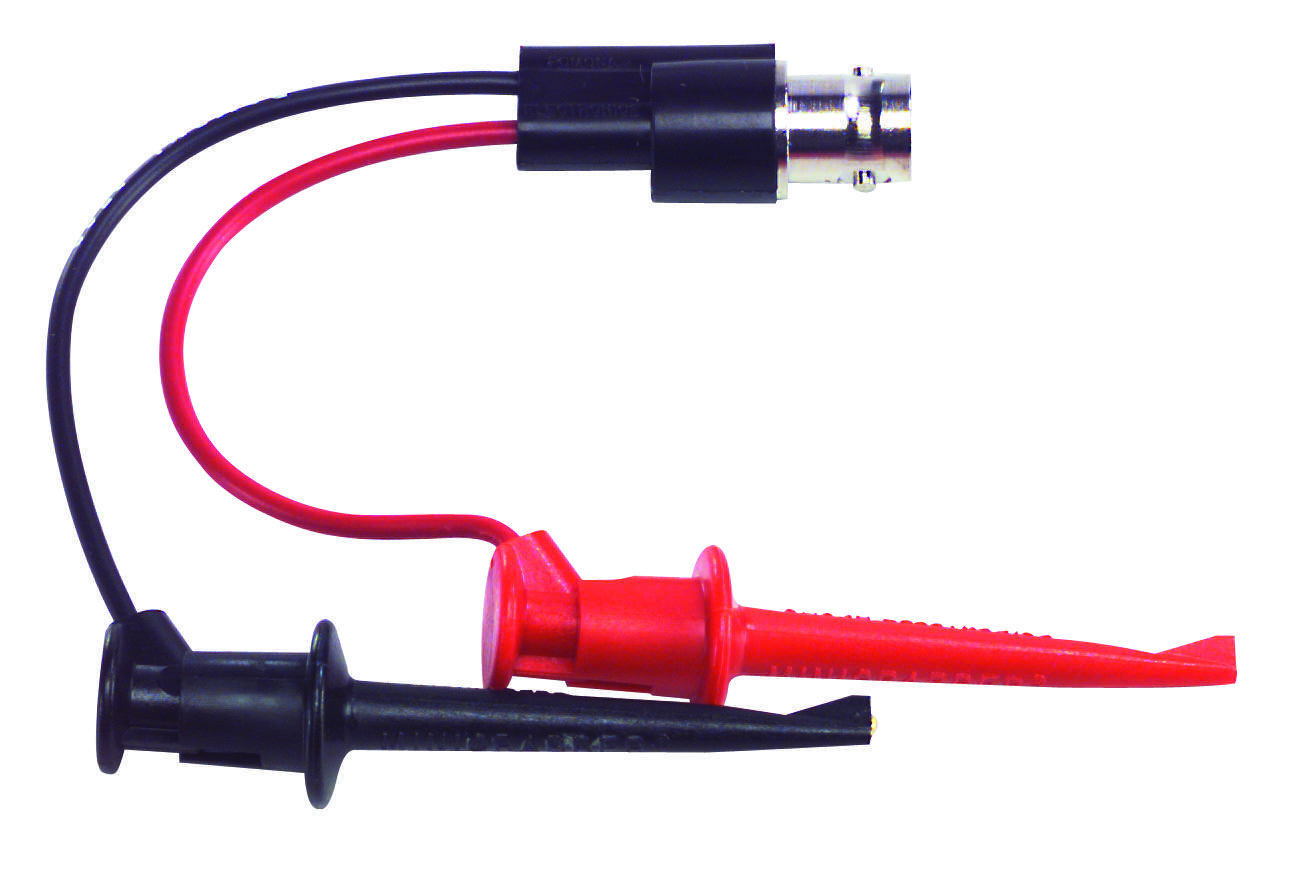
\includegraphics[width=10cm,height=\textheight]{https://raw.githubusercontent.com/kwbunker/PHYS-3330-Scratch/main/lab1fig/mini-grabber-to-bnc.jpg}
\caption{Mini Grabber to BNC Socket Connector}\label{fig:grabber}
}
\end{figure}

\hypertarget{triggering-an-ac-waveform-on-the-scope}{%
\subsection{Triggering an AC waveform on the
scope}\label{triggering-an-ac-waveform-on-the-scope}}

Most scopes produce about 0-5 V square wave on the "PROBE COMP" pins to
use for testing. We will use this to get familiar with triggering the
scope.

\begin{enumerate}
\def\labelenumi{\arabic{enumi}.}
\item
  Connect the Probe Comp output to the scope using mini grabbers (see
  Figure \ref{fig:grabber}).
\item
  Display the waveform on the scope. You will need to trigger the scope
  off of the waveform. Confirm with your instructor that you have the
  scope triggered correctly before continuing. Describe the setup and
  outcomes in your lab notebook.
\end{enumerate}

The trigger level controls the voltage at which the trace starts.
Stability is lost when the trigger level lies outside range of the
displayed voltage. Change TRIGGER MODE to NORMAL. Note that the trace
now "freezes" when the trigger level is misadjusted. You can see whether
or not the scope is actually being triggered by looking for the small
writing TRIGD or TRIG? at the top of the display. \emph{See Appendix for
the trigger menu.}

What is the frequency of the waveform? You can measure the period and
then calculate the frequency using that measurement. Include your
measurements, procedure, and calculations in your lab notebook.

\hypertarget{creating-an-ac-waveform-using-a-function-generator-and-measuring-it-on-a-scope}{%
\subsection{Creating an AC waveform using a function generator and
measuring it on a
scope}\label{creating-an-ac-waveform-using-a-function-generator-and-measuring-it-on-a-scope}}

The Keysight EDU33212A function generator can produce sine, square,
triangle, pulse, and ramp waveforms over the frequencies from 0.000001
Hz to 20 MHz. The output amplitude can be varied between 1 mV and 10 V
peak-to-peak with an output impedance of 50 \(\Omega\).

\textbf{\emph{There is one main precaution to keep in mind: Do not
connect any output of the EDU33212A directly to dc power or to the
output of any other instrument or circuit. Doing so will burn out the
output amplifier!}}

\begin{enumerate}
\def\labelenumi{\arabic{enumi}.}
\item
  Create a 1 V peak-to-peak (p-p) sine wave at 1 kHz with no DC offset
  (you may want to use this standard setup in the future if you have
  trouble). You will need to set the output termination of the function
  generator to HIGH Z (see \emph{Appendix} or page 53 of the User
  Guide).
\item
  Display the waveform on the scope. You can use a BNC cable (see Figure
  \ref{fig:bnc}) to make the connection. You will need to trigger the
  scope off of the waveform.
\item
  Reduce the amplitude to 100 mV p-p.~You may notice the scope stopped
  triggering. This is because the waveform never crosses the trigger
  level now.
\item
  The function generator has a trigger output that can be used to
  trigger the scope (called Sync/Trigger Out). Using the trigger output
  is more convenient than triggering the scope off of the waveform
  itself because you avoid having to readjust the scope trigger every
  time you change the waveform. Connect the Sync output of the function
  generator to Channel 4 of the scope and trigger off of that waveform.
  Now change the amplitude and frequency of the sine wave and notice how
  the scope remains nicely triggered.
\item
  Come up with a waveform of your own that you want to create (e.g.,
  triangle wave at 1 MHz with a 200 mV p-p amplitude) and measure its
  properties with the scope. Report on the one you created and record
  this in your lab notebook. You can either print a screenshot directly
  from the scope or take a picture and print it.
\end{enumerate}

\hypertarget{measuring-quantities-with-the-digital-multimeter}{%
\section{Measuring Quantities with the Digital
Multimeter}\label{measuring-quantities-with-the-digital-multimeter}}

\textbf{The multimeter is a useful device to measure constant voltages,
currents, and resistances.}

To measure various quantities with the DMM, you must set the dial to the
correct setting and verify that the two leads are connected to the
correct input ports.

\begin{enumerate}
\def\labelenumi{\arabic{enumi}.}
\item
  Connect the leads and set the dial to measure resistance. Get five 5k
  (5\%) resistors form the stock drawers. Measure the resistance of each
  resistor. Do all the resistors meet the 5\% specification?
\item
  Connect the leads and set the dial to measure voltage. Measure the
  voltage of both sides of the DC power supply again. Does the measured
  value from the DMM agree with the value indicated on the power supply?
\item
  Connect the leads and set the dial to measure current. Measure the
  current produced by the power supply. \textbf{Make sure the power
  supply current is limited to a value below the fuse of the DMM.} How
  do you experimentally set the current limit? If you blow the fuse,
  just replace it. Does the measured current from the DMM agree with the
  value indicated on the power supply? Using the current and voltage
  readings, what is the impedance of the ammeter? \emph{HINT: The DMM
  leads must be in different places to measure current vs.~voltage.
  Also, it is recommended to use the high current input until you are
  certain that the current is low enough to be read by the low current
  input. This avoids blowing the fuse.}
\item
  The DMM also has an AC voltage setting. Over what frequency range is
  the reading accurate to 2\%? You will need to use the function
  generator to produce an AC waveform. Note: the DMM displays the RMS
  amplitude of the waveform. See Definitions at the beginning of the
  guide for an explanation of RMS.
\item
  Remember in the future that this is the usable frequency range for the
  AC setting of the multimeter. Record this frequency in your lab
  notebook for future reference.
\end{enumerate}

\hypertarget{measuring-small-resistances}{%
\section{Measuring Small
Resistances}\label{measuring-small-resistances}}

In the previous section, you measured resistances using the ohmmeter in
the DMM. You will now use all the measurement techniques and devices you
have learned about to determine most accurate way to measure a small
resistance.

\hypertarget{measure-a-small-resistance-using-a-dmm-ohmmeter}{%
\subsection{Measure a small resistance using a DMM
ohmmeter}\label{measure-a-small-resistance-using-a-dmm-ohmmeter}}

\begin{enumerate}
\def\labelenumi{\arabic{enumi}.}
\item
  Use a \textasciitilde{} 2 m length of magnet wire (26 or 28 gauge) as
  your small resistor. Magnet wire has a very thin amber-colored
  insulating coating. Make sure you remove the insulation from the ends
  of the wire to make a good electrical connection and measurement of
  the diameter of the wire. You can burn off the insulation with a flame
  or carefully scrape it off with a razor blade.
\item
  What is the resistance based on the diameter, length, and resistivity
  (the resistivity, \(\rho\), of copper at room temperature is 1.68
  \(\mu\Omega\)-cm)? Remember that \(R = \rho l/a\), where \(l\) is
  length and \(a\) is area. It is hard to measure the diameter of the
  wire with the insulating coating on and the stripping process usually
  deforms the copper. However, you can just look up the diameter of your
  particular gauge of wire online.
\item
  Use the ohmmeter in the DMM to measure the resistance of the wire.
  \textbf{Document your setup, measurements, and calculations in your
  lab notebook.}
\end{enumerate}

\hypertarget{measure-a-small-resistance-using-a-4-terminal-approach}{%
\subsection{Measure a small resistance using a 4-terminal
approach}\label{measure-a-small-resistance-using-a-4-terminal-approach}}

\begin{enumerate}
\def\labelenumi{\arabic{enumi}.}
\item
  Use your DC power supply to run a current through the wire. You can
  then measure the voltage drop across the wire with a DMM to determine
  its resistance based on Ohms law.
\item
  You can use the display on the power supply to measure the current or
  use your DMM as an ammeter. (Consider the resolution of both devices
  when making your choice.) You can use your DMM as a voltmeter to
  measure the potential difference across the wire. Can you just use the
  voltage reading on the power supply? Explain.
\item
  Draw a diagram of your experimental set up in your lab notebook.
\item
  Consider how the amount of current flowing through your resistor
  affects the sensitivity of your measurement.
\item
  Calculate the resistance of the wire from your measurements using Ohms
  Law.
\end{enumerate}

\hypertarget{compare-the-two-measurement-techniques}{%
\subsection{Compare the two measurement
techniques}\label{compare-the-two-measurement-techniques}}

\begin{enumerate}
\def\labelenumi{\arabic{enumi}.}
\item
  The ohmmeter in the DMM works by supplying a current and measuring the
  potential difference between the outputs. How is this measurement
  different than the 4-terminal approach you built? \emph{Hint: consider
  where the current is flowing and what resistances are involved with
  each measurement technique. It is usually helpful to draw a diagram
  including all the resistances, even of the wires in this case.}
\item
  Which method is more accurate for measuring small resistances based on
  your explanation for part 1?
\item
  Do your two measurements confirm your scientific argument made in part
  2? Defend your assertion using your data.
\end{enumerate}

\hypertarget{summary-and-conclusions}{%
\section{Summary and Conclusions}\label{summary-and-conclusions}}

Write a two-paragraph summary in your lab notebook of what you learned
and any important takeaways.

\hypertarget{appendix-a-tektronix-tbs-2000-series-oscilloscope-controls}{%
\section*{Appendix A: Tektronix TBS 2000 Series Oscilloscope
Controls}\label{appendix-a-tektronix-tbs-2000-series-oscilloscope-controls}}
\addcontentsline{toc}{section}{Appendix A: Tektronix TBS 2000 Series
Oscilloscope Controls}

\textbf{To change the horizontal (time base) scale:}

\begin{enumerate}
\def\labelenumi{\arabic{enumi}.}
\item
  Horizontal scale knob changes the time per division
\item
  Horizontal position knob changes location of the trigger (labeled as a
  orange arrow on the top of the screen)
\end{enumerate}

\textbf{To change the vertical (voltage base) scale:}

\begin{enumerate}
\def\labelenumi{\arabic{enumi}.}
\item
  Vertical scale knob changes the voltage per division
\item
  Vertical position knob changes location of the ground (labeled as a
  colored-coded arrow on the left of the screen)
\end{enumerate}

\textbf{To access the parameters for each channel:}

Ch. 1 (or 2,3,4) button \textgreater{} Vertical MENU button (under
Vertical Scale knob)

\begin{enumerate}
\def\labelenumi{\arabic{enumi}.}
\item
  Input Coupling (AC/DC/Ground)
\item
  Invert Signal
\item
  Probe Setup
\item
  Input Impedance (1M\(\Omega\) or 50\(\Omega\))
\end{enumerate}

Ch. 1 (or 2,3,4) button Vertical Off button (above Vertical Scale knob)

\begin{enumerate}
\def\labelenumi{\arabic{enumi}.}
\tightlist
\item
  turns off that channels trace
\end{enumerate}

\textbf{To adjust the trigger:}

\begin{enumerate}
\def\labelenumi{\arabic{enumi}.}
\item
  Trigger knob changes the voltage level of the trigger
\item
  Trigger MENU button

  a. Select which channel to trigger off of (trigger level arrow changes
  color to show which channel is being triggered)

  b. Slope: can trigger off a rising or falling edge.

  c. Trigger Mode: Auto, Normal, other
\end{enumerate}

\textbf{To select the AQUIRE mode:}

\begin{enumerate}
\def\labelenumi{\arabic{enumi}.}
\item
  Run/Stop: sets the scope to continuously quire or freeze after last
  trigger
\item
  Single sequence: draws once after it triggers
\item
  Autoset: scope tries to choose overall best scope settings (sometimes
  useful when you cant see anything, but generally used as a last resort
  because it can also mislead you )
\end{enumerate}

\textbf{Measure Menu (top of panel):}

You can select various measurements and which channel to measure.
\emph{Be very careful} with automatic measurements (again these can be
deceptive). Generally use cursors to make accurate measurements. Note
that the automatic mode searches for the very top and bottom of the
signals. For example, in the schematic of a noisy sine wave below,
automatic mode will return the upper and lower most lines which will
include the noise contribution. A careful manual measurement indicated
by the inner (shorter) lines can remove the noise from the amplitude
measurement. \textbf{With small or noisy signals, the automatic mode
will give very poor results.}

\textbf{Cursor Menu (top of panel):}

\begin{enumerate}
\def\labelenumi{\arabic{enumi}.}
\item
  Choose time (vertical bars) or voltage (horizontal bars) measurement.
\item
  Choose which channel to measure (measurement cursors are the same
  color as the channel they are measuring)
\item
  Big top knob moves the cursors
\item
  SELECT button changes which cursor to move.
\item
  Position relative to ground (trigger zero time) is displayed on the
  screen with the "@" symbol.
\item
  Relative distance between cursors is displayed on the screen with the
  \(\Delta\) symbol.
\end{enumerate}

\hypertarget{appendix-b-changing-the-output-termination-on-the-function-generator-keysight-edu33212a}{%
\section*{Appendix B: Changing the Output Termination on the Function
Generator (Keysight
EDU33212A)}\label{appendix-b-changing-the-output-termination-on-the-function-generator-keysight-edu33212a}}
\addcontentsline{toc}{section}{Appendix B: Changing the Output
Termination on the Function Generator (Keysight EDU33212A)}

\begin{enumerate}
\def\labelenumi{\arabic{enumi}.}
\item
  Press a channel {[}Setup{]} key to open the channel configuration
  screen. Note that the current output termination values (both 50
  \(\Omega\) in this case) appear on the tabs at the top of the screen.

  \begin{fignos:no-prefix-figure-caption}

  \begin{figure}
  \centering
  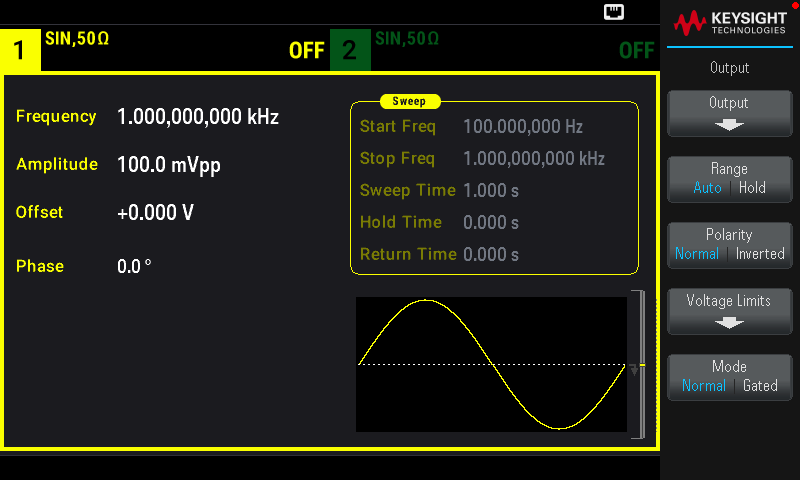
\includegraphics[width=10cm,height=\textheight]{https://raw.githubusercontent.com/kwbunker/PHYS-3330-Scratch/main/lab1fig/EDU33212A-term1.png}
  \caption{}
  \end{figure}

  \end{fignos:no-prefix-figure-caption}
\item
  Begin specifying the output termination by pressing Output.

  \begin{fignos:no-prefix-figure-caption}

  \begin{figure}
  \centering
  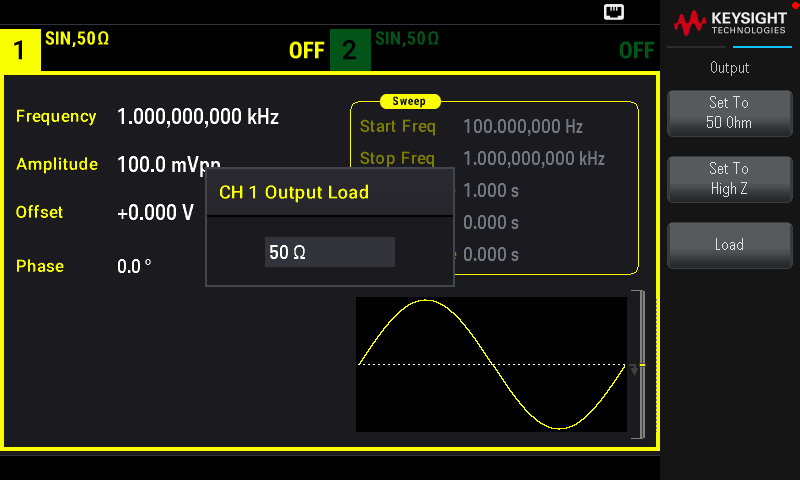
\includegraphics[width=10cm,height=\textheight]{https://raw.githubusercontent.com/kwbunker/PHYS-3330-Scratch/main/lab1fig/EDU33212A-term2.png}
  \caption{}
  \end{figure}

  \end{fignos:no-prefix-figure-caption}
\item
  Select the desired output termination either by using the knob or
  numeric keypad to select the desired load impedance or by pressing Set
  to 50 \(\Omega\) or Set to High Z. You can also set a specific value
  by pressing Load.

  \begin{fignos:no-prefix-figure-caption}

  \begin{figure}
  \centering
  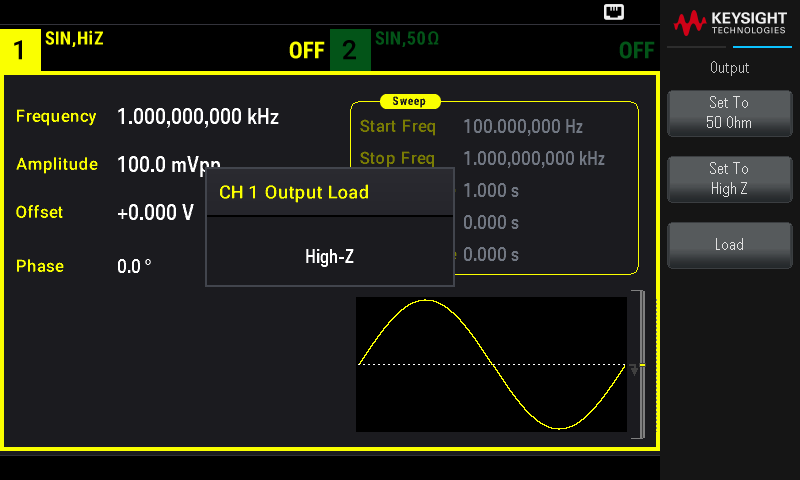
\includegraphics[width=10cm,height=\textheight]{https://raw.githubusercontent.com/kwbunker/PHYS-3330-Scratch/main/lab1fig/EDU33212A-term3.png}
  \caption{}
  \end{figure}

  \end{fignos:no-prefix-figure-caption}
\end{enumerate}

\end{document}
